% Capítulo 8: heap máximo como árvore e como vetor.
\documentclass[border=4pt]{standalone}
\usepackage[utf8]{inputenc}
\usepackage[T1]{fontenc}
% Estilo comum das figuras de vetores (capítulo 8).
\usepackage{tikz}
\usetikzlibrary{arrows.meta, positioning, calc, decorations.pathreplacing}
\definecolor{navy}{RGB}{23,45,80}
\definecolor{laranja}{RGB}{250,110,29}
\definecolor{cinzalogo}{RGB}{107,114,126}
\definecolor{azul}{RGB}{205,222,247}
\tikzset{
  casa/.style={draw=navy, line width=0.9pt, minimum width=8mm, minimum height=7mm,
               inner sep=0pt, font=\sffamily\small},
  pronta/.style={casa, fill=azul},
  parte/.style={casa, fill=laranja!12},
  marcada/.style={casa, fill=laranja!45, draw=laranja},
  fora/.style={casa, draw=cinzalogo!60, dashed, fill=white, text=cinzalogo!60},
  indice/.style={font=\sffamily\scriptsize, text=cinzalogo},
  explica/.style={font=\sffamily\small, text=navy, anchor=east},
  legenda/.style={font=\sffamily\scriptsize, text=cinzalogo},
  rotulo/.style={font=\sffamily\small\bfseries, text=navy},
  seta/.style={-{Stealth[length=2.2mm]}, navy, line width=0.9pt},
  chave/.style={decorate, decoration={brace, amplitude=4pt, mirror}, navy, line width=0.8pt},
}
% \vetor{nome}{x}{y}{valor/estilo, valor/estilo, ...}: casas lado a lado, chamadas nome0, nome1...
\newcommand{\vetor}[4]{%
  \foreach \valor/\estilo [count=\i from 0] in {#4} {
    \node[\estilo] (#1\i) at ($(#2, #3) + (\i*0.8, 0)$) {\valor};
  }
}

\tikzset{
  no/.style={circle, draw=navy, line width=0.9pt, fill=laranja!12, minimum size=8mm,
             inner sep=0pt, font=\sffamily\small},
  raiz/.style={no, fill=laranja!45, draw=laranja},
  aresta/.style={draw=navy, line width=0.9pt},
}
\begin{document}
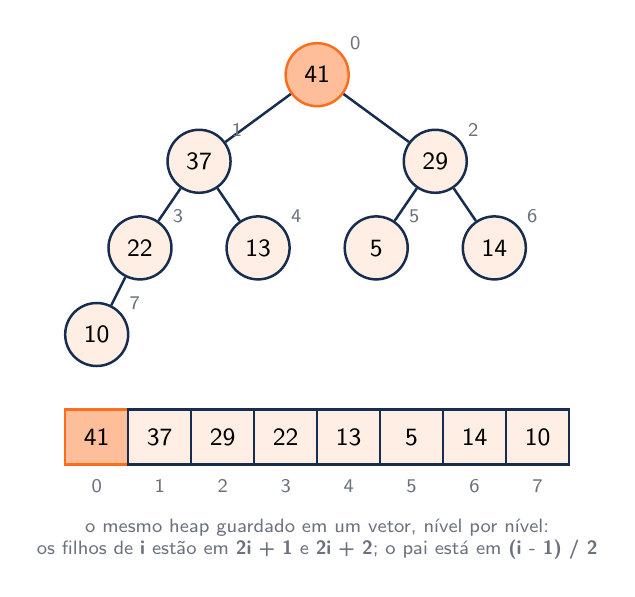
\begin{tikzpicture}
  \node[raiz] (n0) at (3, 0) {41};
  \node[no] (n1) at (1.5, -1.1) {37};
  \node[no] (n2) at (4.5, -1.1) {29};
  \node[no] (n3) at (0.75, -2.2) {22};
  \node[no] (n4) at (2.25, -2.2) {13};
  \node[no] (n5) at (3.75, -2.2) {5};
  \node[no] (n6) at (5.25, -2.2) {14};
  \node[no] (n7) at (0.2, -3.3) {10};
  \foreach \p/\f in {0/1, 0/2, 1/3, 1/4, 2/5, 2/6, 3/7} { \draw[aresta] (n\p) -- (n\f); }
  \foreach \i in {0,...,7} { \node[indice, above right=-1mm and 0mm of n\i] {\i}; }
  \vetor{v}{0.2}{-4.6}{41/marcada, 37/parte, 29/parte, 22/parte, 13/parte, 5/parte, 14/parte, 10/parte}
  \foreach \i in {0,...,7} { \node[indice, below=0.5mm of v\i] {\i}; }
  \node[legenda, align=center] at (3, -5.9)
    {o mesmo heap guardado em um vetor, nível por nível:\\
     os filhos de \textbf{i} estão em \textbf{2i + 1} e \textbf{2i + 2}; o pai está em \textbf{(i - 1) / 2}};
\end{tikzpicture}
\end{document}
